\documentclass[11pt, twoside]{book}

\ifx\pdfoutput\undefined
% we are running LaTeX, not pdflatex
\usepackage{graphicx}
\else
% we are running pdflatex, so convert .eps files to .pdf
\usepackage[pdftex]{graphicx}
\usepackage{epstopdf}
\fi

%\usepackage[cp1252]{inputenc} % soportes para acentos 
\usepackage[spanish,activeacute,english]{babel}  % texto autogenerado en espaol
%\usepackage[latin1]{inputenc}
\usepackage{ucs}
\usepackage[utf8]{inputenc} % Para linux, utf8
\usepackage{fontenc} 
%\usepackage[T2A]{fontenc} 
\usepackage[T1]{fontenc} 
\usepackage{geometry} % figuras

\usepackage{titlesec} % Soporte para modificar apariencia de los titulos 
%\usepackage{fancyhdr}       % Soporte para los encabezados de pagina 
\usepackage{anysize}        % Soporte para el comando \marginsize 
\usepackage{url}
\usepackage{multirow}
\usepackage{subfig}
%\usepackage{fancyvrb}
%\usepackage{verbatim}
\usepackage{listings}
\usepackage{color}

%\usepackage[nottoc]{tocbibind} 
\usepackage{hyperref} 
\usepackage{listings} 
\usepackage{float} 
\usepackage{amsmath} 

\usepackage{enumerate}

\usepackage{minted}
%\usemintedstyle{tango}

%%%%%%%%%%%%%%%%%%%%%%%%%%%%%%%%%%%%%%%%%%%%%%%%%%%%%%%%%%%%%%%%%%%%%%%%%%%%%%%%
% CAPTIONS
%%%%%%%%%%%%%%%%%%%%%%%%%%%%%%%%%%%%%%%%%%%%%%%%%%%%%%%%%%%%%%%%%%%%%%%%%%%%%%%%
\usepackage{caption}
\captionsetup{font=footnotesize,labelfont=bf}

%%%%%%%%%%%%%%%%%%%%%%%%%%%%%%%%%%%%%%%%%%%%%%%%%%%%%%%%%%%%%%%%%%%%%%%%%%%%%%%%
% HEADERS
%%%%%%%%%%%%%%%%%%%%%%%%%%%%%%%%%%%%%%%%%%%%%%%%%%%%%%%%%%%%%%%%%%%%%%%%%%%%%%%%
\usepackage{fancyhdr}
\pagestyle{fancy}
 \fancyhead{}
 \fancyhead[RE]{\footnotesize{ \leftmark}}
 \fancyhead[LO]{\footnotesize{ \rightmark}}
\fancyfoot{}
\fancyfoot[LE]{\thepage}
\fancyfoot[RO]{\thepage}

% Code for creating empty pages
% No headers on empty pages before new chapter
\makeatletter
\def\cleardoublepage{\clearpage\if@twoside \ifodd\c@page\else
    \hbox{}
    \thispagestyle{plain}
    \newpage
    \if@twocolumn\hbox{}\newpage\fi\fi\fi}
\makeatother \clearpage{\pagestyle{plain}\cleardoublepage}

\makeatletter
\def\cleardoublepageempty{\clearpage\if@twoside \ifodd\c@page\else
    \hbox{}
    \thispagestyle{empty}
    \newpage
    \if@twocolumn\hbox{}\newpage\fi\fi\fi}
\makeatother \clearpage{\pagestyle{plain}\cleardoublepage}

%%%%%%%%%%%%%%%%%%%%%%%%%%%%%%%%%%%%%%%%%%%%%%%%%%%%%%%%%%%% 
% TITLES
%%%%%%%%%%%%%%%%%%%%%%%%%%%%%%%%%%%%%%%%%%%%%%%%%%%%%%%%%%%% 
\newcommand{\bigrule}{\titlerule[0.5mm]} 

%\usepackage[Lenny]{fncychap}

\titleformat{\chapter}[display] 
{\bfseries\Huge} 
{%\titlerule 
\filright 
\Huge\chaptertitlename\ 
\Huge\thechapter 
} 
{1mm} 
{\filright} 
[\vspace{0.5mm} \bigrule] 

\bibliographystyle{plain}


% So the code looks nice
\definecolor{gray97}{gray}{.97}
\definecolor{gray75}{gray}{.75}
\definecolor{gray45}{gray}{.45}

%%%%%%%%%%%%%%%%%%%%%%%%%%%%%%%%%%%%%%%%%%%%%%%%%%%%%%%%%%%%%%%%%%%%%%%%%%%%%%%%
% SOURCE CODE
%%%%%%%%%%%%%%%%%%%%%%%%%%%%%%%%%%%%%%%%%%%%%%%%%%%%%%%%%%%%%%%%%%%%%%%%%%%%%%%%

% Load languages
\lstloadlanguages{Ruby,sh}

\lstset{
   frame=Ltb,
   framerule=0pt,
   aboveskip=0.5cm,
   framextopmargin=3pt,
   framexbottommargin=3pt,
   framexleftmargin=0.4cm,
   framesep=0pt,
   rulesep=.4pt,
   rulesepcolor=\color{black},
   %
   stringstyle=\ttfamily,
   showstringspaces = false,
   basicstyle=\small\ttfamily,
   commentstyle=\color{gray45},
   keywordstyle=\bfseries,
   %
   breaklines=true,
   }
 
\lstnewenvironment{bash}[1][]
   {\lstset{language=sh,
            backgroundcolor=\color{gray97},}}
   {}
   
\lstnewenvironment{ruby}[1][]
   {\lstset{language=Ruby,
            backgroundcolor=\color{white},
            numbers=left,
            numbersep=15pt,
            numberstyle=\tiny,
            numberfirstline = false,}}
   {}

\definecolor{bg}{rgb}{0.95,0.95,0.95}
\newminted{ruby}{linenos,frame=single}
\newminted{yaml}{frame=lines}
\newminted{bash}{bgcolor=bg,frame=single}

%%%%%%%%%%%%%%%%%%%%%%%%%%%%%%%%%%%%%%%%%%%%%%%%%%%%%%%%%%%%%%%%%%%%%%%%%%%%%%%%
% TABLE OF CONTENTS & BIBLIOGRAPHY
%%%%%%%%%%%%%%%%%%%%%%%%%%%%%%%%%%%%%%%%%%%%%%%%%%%%%%%%%%%%%%%%%%%%%%%%%%%%%%%%
% Numeramos hasta 3 niveles y los incluimos en la tabla de contenidos
\setcounter{secnumdepth}{3}
\setcounter{tocdepth}{3}

% Para que ponga 'tabla' en vez de 'cuadro'
% y la bibliografía se llame 'Bibliografía'
\addto\captionsspanish{%
\def\bibname{Bibliografía}
\def\tablename{Tabla}%
\def\listtablename{Índice de tablas}
}

%%%%%%%%%%%%%%%%%%%%%%%%%%%%%%%%%%%%%%%%%%%%%%%%%%%%%%%%%%%%%%%%%%%%%%%%%%%%%%%%
% DOCUMENT
%%%%%%%%%%%%%%%%%%%%%%%%%%%%%%%%%%%%%%%%%%%%%%%%%%%%%%%%%%%%%%%%%%%%%%%%%%%%%%%%
\begin{document}

\selectlanguage{spanish}

\renewcommand{\listtablename}{Índice de tablas}
\renewcommand{\bibname}{Bibliografía}

\begin{titlepage} 
\begin{center} 
 
\includegraphics*[height=3.5cm]{imagenes/logo.png}\\ 

\vspace*{1.5cm} 
{\large Proyecto Fin de Carrera}\\ 
\vspace*{0.2cm} 
{\large Ingeniería en Informática}\\ 
\vspace*{1.5cm} 
{\huge \textbf{Diseño e implementación de un sistema de ejecución de trabajos distribuidos\\}}
\vspace*{2cm} 
{\Large \textbf{David Ceresuela Palomera\\}}
\vspace*{2cm} 
{\normalsize Director: Javier Celaya}\\ 
\vspace*{1.5cm} 
{\normalsize Departamento de Informática e Ingeniería de Sistemas}\\ 
{Escuela de Ingeniería y Arquitectura}\\ 
{Universidad de Zaragoza}\\ 
\vspace*{3.5cm} 
{\normalsize Curso 2011/2012}\\ 
{\normalsize Junio 2012}\\ 
\end{center} 
\end{titlepage} 

\cleardoublepageempty

\selectlanguage{spanish}

\frontmatter % numeración romana, capítulos aparecen en la tabla de contenidos

\chapter{Resumen}
\label{cap:resumen}


A la hora de ejecutar trabajos en un entorno distribuido la aproximación clásica ha sido bien el uso de un \emph{cluster} de ordenadores o bien el uso de la computación en malla o \emph{grid}. Con la proliferación de entornos \emph{cloud} durante estos últimos años y su facilidad de uso, parece que una nueva opción se abre para la ejecución de este tipo de trabajos.\\

De hecho, la ejecución de trabajos distribuidos es uno de los principales usos dentro del ámbito de los sistemas \emph{cloud}. Sin embargo, la administración de este tipo de sistemas dista de ser sencilla: cuestiones como la puesta en marcha del sistema, el aprovisionamiento de nodos, las modificaciones del sistema y la evolución y actualización del mismo suponen una tarea intensa y pesada.\\

En vista de lo cual, en este proyecto se ha diseñado una solución capaz de automatizar la administración de sistemas \emph{cloud}, y en particular de un sistema de ejecución de trabajos distribuidos. Para ello se han estudiado entornos clásicos de ejecución de trabajos como Torque y entornos de ejecución de trabajos en \emph{cloud} como AppScale. Además, se han estudiado herramientas clásicas de configuración automática de sistemas como Puppet y CFEngine. El objetivo principal de estas herramientas de configuración de sistemas es la gestión del nodo. En este proyecto se ha extendido la funcionalidad de una de estas herramientas -- Puppet -- añadiéndole la capacidad de gestión de sistemas \emph{cloud}.\\

Como resultado de este proyecto se presenta una solución capaz de administrar de forma automática sistemas de ejecución de trabajos distribuidos. La validación de esta solución se ha llevado a cabo sobre los entornos de ejecución de trabajos Torque y AppScale y también, para mostrar su carácter genérico, sobre una arquitectura de servicios web de tres niveles.


\tableofcontents
%\listoftables
%\listoffigures

%chapters
\mainmatter % numeración arábiga

\chapter{Introducción}
\label{cap:introduccion}


Durante los últimos años la computación en la nube ha ido ganando importancia de manera progresiva. La capacidad de usar la computación como un servicio permite a los usuarios finales de una aplicación acceder a ésta a través de un navegador web, una aplicación móvil o un cliente de escritorio mientras que la lógica de la aplicación y los datos se encuentran en servidores situados en una localización remota. Las aplicaciones en la nube tratan de proporcionar al usuario el mismo servicio y rendimiento que las aplicaciones instaladas localmente en su ordenador.\\

A lo largo de este proyecto se verán tres ejemplos de infraestructuras distribuidas. La primera de ellas es la infraestrucutra de ejecución de trabajos. Este tipo de infraestructuras está especializada en la ejecución de grandes cargas de trabajo paralelizable e intensivo en computación. Son por lo tanto idóneas para ser usadas en la computación de altas prestaciones. Dentro de esta infraestructura distribuida los ejemplos más claros que podemos encontrar son Condor y Torque.

La segunda infraestructura es la de servicios web en tres capas. Este tipo de infraestructuras tiene tres niveles claramente diferenciados: balanceo o distribución de carga, servidor web y base de datos. El primer nivel de esta arquitectura es el encargado de distribuir la carga (las peticiones web) a los elementos del segundo nivel. Éstos procesarán las peticiones web y para ello puede que tengan que consultar o modificar ciertos datos. Los datos de la aplicación se encuentran en el tercer nivel, y  por consiguiente, cada vez que uno de los elementos del segundo nivel necesite leer información de la base de datos o modificarla, accederá a este tercer nivel. En esta infraestructura no hay un ejemplo claro, pero cualquier página web profesional de hoy en día se sustenta en una arquitectura similar a ésta.

La tercera y última es AppScale, una implementación \emph{open source} del App Engine de Google. App Engine permite alojar aplicaciones web en la infraestructura que Google posee. Además de presentar esta funcionalidad AppScale también ofrece las APIs de EC2, MapReduce y Neptune. La API de EC2 añade a las aplicaciones la capacidad de interactuar con máquinas alojadas en Amazon EC2. La API de MapReduce permite escribir aplicaciones que hagan uso del \emph{framework} (o paradigma?) MapReduce. La última API, Neptune, añade a App Engine la capacidad de usar los nodos de la infraestructura para ejecutar trabajos. Los trabajos más representativos que puede ejecutar son: de entrada, de salida y MPI. El trabajo de entrada sirve para subir ficheros (generalmente el código que se ejecutará) a la infraestructura, el de salida para traer ficheros (generalmente los resultados obtenidos después de la ejecución) y el de MPI para ejecutar un trabajo MPI.

La infraestructura necesaria para dar soporte a todas estas APIs ya no es tan sencilla como en los dos casos anteriores. De hecho, las anteriores infraestructuras estarían contenidas en ésta. Hay dos maneras de definir la infraestructura de AppScale. En la primera de ellas se define un despliegue por defecto, en el que un nodo toma el rol de \emph{controller} y el resto de nodos toman el rol de \emph{servers}. El nodo \emph{controller} es el que carga con la responsabilidad de la coordinación y los nodos \emph{servers} son los que llevan cabo la mayor parte del trabajo. La segunda manera de definir la infraestructura es hacerlo a través de un despliegue personalizado. En este despliegue podemos definir con más precisión los roles que queremos que desempeñe un nodo. Entre todos los posibles roles que AppScale ofrece, los más interesantes desde nuestro punto de vista son: \emph{master}, \emph{appengine}, \emph{database}, \emph{login} y \emph{open}.\\

De igual manera, las herramientas de administración de sistemas (o herramientas de gestión de configuración) también han experimentado un considerable avance. Con entornos cada vez más heterogéneos y complejos la administración de sistemas de manera manual ya no es una opción. Entre todo el conjunto de  herramientas destacan de manera especial Puppet y CFEngine. Puppet es una herramienta de gestión de configuración basada en un lenguaje  declarativo: el usuario especifica qué estado debe alcanzarse y Puppet se encarga de hacerlo. CFEngine permite al usuario un control más fino de cómo se hacen las cosas, ganando velocidad a costa de perder elementos de más alto nivel.\\

Sin embargo, estas herramientas de gestión de la configuración carecen de la funcionalidad requerida para administrar infraestructuras distribuidas.\\

Si tomamos la administración de un cloud como la administración de las MV que forman los nodos del cloud nos damos cuenta de que la administración es puramente software.\\


\section{Contexto del proyecto}

Para la realización de este proyecto de fin de carrera se ha hecho uso del laboratorio 1.03b de investigación que el Departamento de Informática e Ingeniería de Sistemas posee en la Escuela de Ingeniería y Arquitectura de la Universidad de Zaragoza. Los ordenadores que forman este laboratorio poseen procesadores con soporte de virtualización, lo que permite la creación de diversas máquinas virtuales. La creación de los distintos tipos de cloud que representan cada una de las infraestructuras distribuidas se ha llevado a cabo a través de máquinas virtuales alojadas en distintos ordenadores del laboratorio.\\

En este laboratorio se ha comprobado la validez de la extensión para administración de clouds introducida en la herramienta de gestión de configuraciones Puppet que se ha desarrollado a lo largo del proyecto de fin de carrera.


\section{Objetivos}

El objetivo de este proyecto es proporcionar una herramienta que facilite la puesta en marcha de infraestructuras distribuidas y su posterior mantenimiento. Las tareas principales en las que se puede dividir este proyecto son:

\begin{enumerate}
\item Estudio de algunas de las infraestructuras distribuidas existentes profundizando en la parte relativa a la ejecución de trabajos distribuidos.
\item Análisis de las herramientas de administración de virtualización \emph{hardware}.
\item Investigación de las herramientas de gestión de configuración existentes más relevantes y elección de aquella que mayor facilidad de integración y uso proporcione.
\item Extensión de la herramienta de gestión de configuración para que soporte la puesta en marcha y el mantenimiento de un sistema de ejecución de trabajos distribuidos.
\end{enumerate}


\section{Organización de la memoria}

El resto de este documento queda organizado de la siguiente manera:
\begin{description}
\item[Capítulo \ref{cap:trabajo}] Extensión de Puppet para soporte de infraestructuras distribuidas.
\item[Capítulo \ref{cap:appscale}] Uso de la extensión de Puppet para soporte de infraestructura AppScale.
\item[Capítulo \ref{cap:web}] Uso de la extensión de Puppet para soporte de infraestructura web de tres niveles.
\item[Capítulo \ref{cap:torque}] Uso de la extensión de Puppet para soporte de infraestructura de trabajos distribuidos.
\item[Capítulo \ref{cap:conclusiones}] Conclusiones.
\end{description}


\section{Agradecimientos}

Agradecimientos

\chapter{Metodología de diseño e implementación de recursos distribuidos}
\label{cap:metodologia}

Una vez que el modelado se ha completado es tiempo de abarcar la metodología que se sigue a la hora de diseñar e implementar nuevos recursos distribuidos. Para ello se usan las facilidades que proporciona la herramienta de gestión de configuración para ampliar su funcionalidad.


%%%%%%%%%%%%%%%%%%%%%%%%%%%%%%%%%%%%%%%%%%%%%%%%%%%%%%%%%%%%%%%%%%%%%%%%%%%%%%%%
\section{Especificación del tipo}

El primer paso que hay que hacer a la hora de crear un nuevo recurso en Puppet es definir el tipo de recurso. Para ello en un fichero habrá que especificar el nombre del nuevo tipo y los argumentos que éste tiene. Durante esta sección y la siguiente se usará el ejemplo de la arquitectura web de tres niveles ya que es la más conocida y sirve para demostrar que el enfoque que se ha tomado es lo suficientemente general y válido también para infraestructuras que nada tienen que ver con la ejecución de trabajos. \\

Una típica arquitectura de servicios web consta de al menos tres niveles: balanceo de carga, servidores web y base de datos. Cada uno de estos niveles está compuesto por al menos un elemento clave: el balanceador de carga, el servidor web y el servidor de base de datos, respectivamente. El balanceador de carga es el punto de entrada al sistema y el que se encarga, como su nombre indica, de repartir las peticiones de los clientes a los distintos servidores web. Los servidores web se encargan de servir las páginas web a los clientes y para ello, dependiendo de las peticiones que hagan los clientes, podrán leer o almacenar información en la base de datos. Para manipular dicha información los servidores web tendrán que comunicarse con el servidor de base de datos, que es el que hará efectiva la lectura y modificación de la información.\\

\begin{figure} [!htbp]
  \centering
  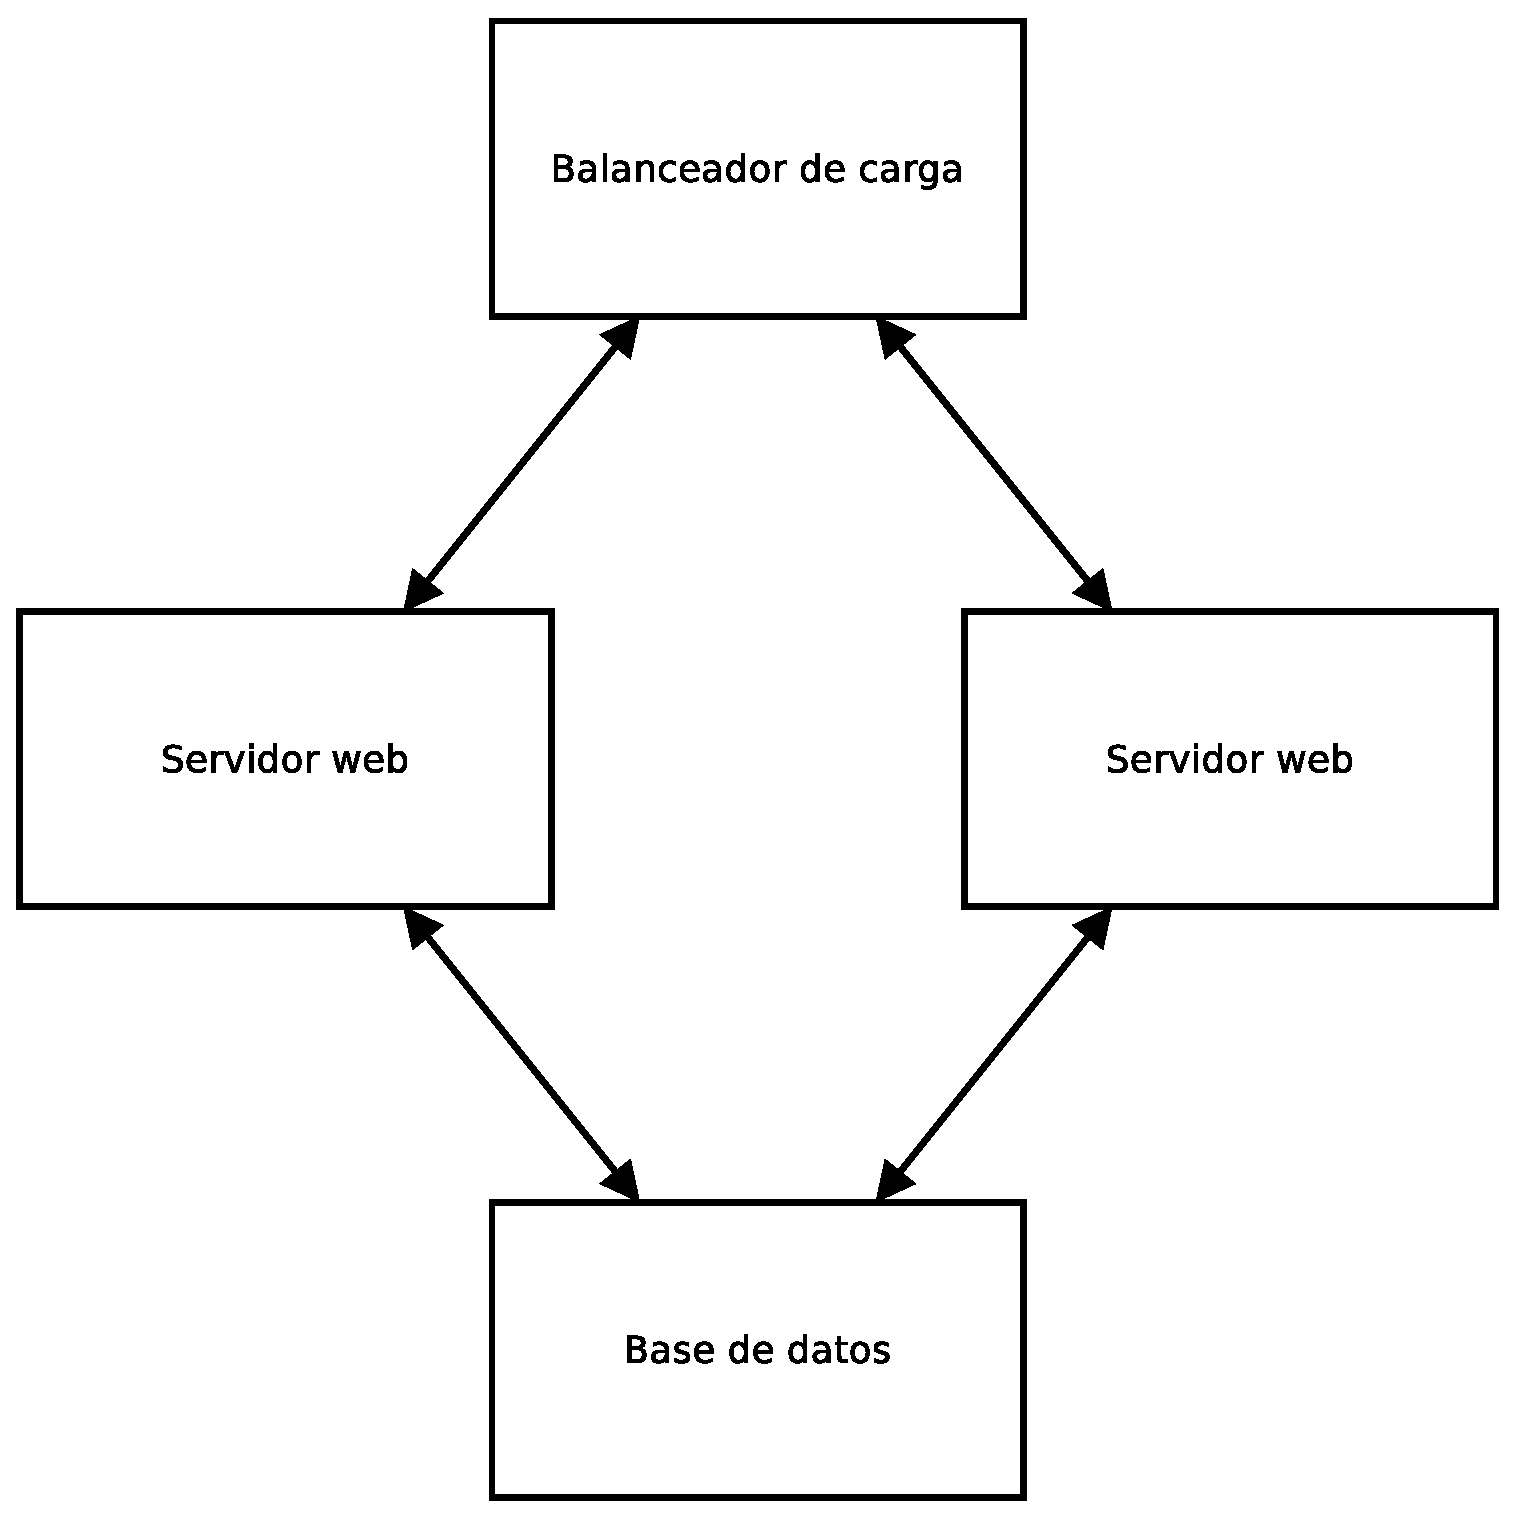
\includegraphics[width=0.5\textwidth]{figuras/Arquitectura_Web2.eps}
  \caption{Infraestructura web de tres niveles.}
\label{figure:arquitectura-web}
\end{figure}

La infraestructura usada como ejemplo consta de un balanceador de carga, dos servidores web y un servidor de bases de datos (Figura \ref{figure:arquitectura-web}).


\pagebreak

La creación del tipo \texttt{web} se hace en el fichero \texttt{web.rb}, en el lugar apropiado dentro del correspondiente módulo. En el siguiente fragmento de código se indican los aspectos más importantes (la implementación completa puede encontrarse en el Anexo \ref{anx:codigo}) del mismo:

\begin{rubycode}
Puppet::Type.newtype(:web) do
   @doc = "Manages web clouds formed by KVM virtual machines."
   
   
   ensurable do

      desc "The cloud's ensure field can assume one of the following values:
   `running`: The cloud is running.
   `stopped`: The cloud is stopped.\n"
   
      newvalue(:stopped) do
         provider.stop
      end

      newvalue(:running) do
         provider.start
      end

   end


   # General parameters
   
   newparam(:name) do
      desc "The cloud name"
      isnamevar
   end
   
   newparam(:vm_domain) do
      desc "The XML file with the virtual machine domain definition. " +
           "Libvirt XML format must be used"
   end
   
   newproperty(:pool, :array_matching => :all) do
      desc "The pool of physical machines"
   end

   # ...


   # Web parameters
   
   newproperty(:balancer, :array_matching => :all) do
      desc "The balancer node's information"
   end
   
   newproperty(:server, :array_matching => :all) do
      desc "The server nodes' information"
   end
   
   newproperty(:database, :array_matching => :all) do
      desc "The database node's information"
   end

end

\end{rubycode}

Dentro del tipo \texttt{web}, los atributos \texttt{name}, \texttt{vm\_domain} y \texttt{pool} se corresponden con los atributos \texttt{Nombre}, \texttt{Fichero de dominio} y \texttt{Conjunto de máquinas físicas} definidos en la sección \ref{sec:modelado-puppet}. Los atributos \texttt{balancer}, \texttt{server} y \texttt{database} son los atributos propios de la arquitectura web.

Una vez que el tipo está definido, ya se puede ver cuál será el aspecto de un manifiesto para un recurso de tipo web:

%%% Revisar que no cambie

\begin{lstlisting}
web {'mycloud':
   balancer  => ["155.210.155.175", "/var/tmp/dceresuela/lucid-lb.img"],
   server    => ["/etc/puppet/modules/web/files/server-ips.txt",
                 "/etc/puppet/modules/web/files/server-imgs.txt"],
   database  => ["155.210.155.177", "/var/tmp/dceresuela/lucid-db.img"],
   vm_domain => "/etc/puppet/modules/web/files/mycloud-template.xml",
   pool      => ["155.210.155.70"],
   ensure    => running,
}
\end{lstlisting}

%%%%%%%%%%%%%%%%%%%%%%%%%%%%%%%%%%%%%%%%%%%%%%%%%%%%%%%%%%%%%%%%%%%%%%%%%%%%%%%%
\section{Diseño e implementación del proveedor}

Después de haber definido el tipo del recurso, queda definir el proveedor que implementa dicho tipo. En el caso de los recursos distribuidos, y teniendo en cuenta las funciones de arranque y parada especificadas en el tipo (en el bloque \texttt{ensurable}, líneas 5 a 19), el proveedor deberá contener obligatoriamente las funciones \texttt{start} y \texttt{stop}. A continuación se presenta un proveedor con los aspectos más importantes (la implementación completa se encuentra en el Anexo \ref{anx:codigo}):

\begin{rubycode}
Puppet::Type.type(:web).provide(:webp) do
   desc "Manages web clouds formed by KVM virtual machines"

   # Require files
   # ...

   # Start function. Makes sure the cloud is running.
   def start
   
      cloud = Cloud.new(CloudInfrastructure.new(), CloudLeader.new(), resource,
                        method(:err))
      puts "Starting cloud %s" % [resource[:name]]
      
      # Check existence
      if !exists?
         # Cloud does not exist => Startup operations
         
         # Check pool of physical machines
         puts "Checking pool of physical machines..."
         pm_up, pm_down = cloud.check_pool()
         unless pm_down.empty?
            puts "Some physical machines are down"
            pm_down.each do |pm|
               puts " - #{pm}"
            end
         end
         
         # Obtain the virtual machines' IPs
         puts "Obtaining the virtual machines' IPs..."
         vm_ips, vm_ip_roles, vm_img_roles = obtain_vm_data(cloud.resource)
         
         # Check whether you are one of the virtual machines
         puts "Checking whether this machine is part of the cloud..."
         part_of_cloud = vm_ips.include?(MY_IP)
         if part_of_cloud
            puts "#{MY_IP} is part of the cloud"
            
            # Check if you are the leader
            if cloud.leader?()
               cloud.leader_start("web", vm_ips, vm_ip_roles, vm_img_roles,
                                  pm_up, method(:web_monitor))
            else
               cloud.common_start()
            end
         else
            puts "#{MY_IP} is not part of the cloud"
            cloud.not_cloud_start("web", vm_ips, vm_ip_roles, vm_img_roles,
                                  pm_up)
         end
         
      else
         
         # Cloud exists => Monitoring operations
         puts "Cloud already started"
         
         # Check if you are the leader
         if cloud.leader?()
            cloud.leader_monitoring(method(:web_monitor))
         else
            puts "#{MY_IP} is not the leader"      # Nothing to do
         end
      end
      
   end


   # Stop function. Makes sure the cloud is not running.
   def stop

      # ...
   
   end


   def status
      if File.exists?("/tmp/cloud-#{resource[:name]}")
         return :running
      else
         return :stopped
      end
   end
   
end
\end{rubycode}

Son especialmente importantes dentro de este proveedor las líneas 10, 30 y 40. En la línea 10 creamos un nuevo objeto de la clase \texttt{Cloud} (\ref{sec:modelado-framework}). En la línea 30 se llama a la función \texttt{obtain\_vm\_data} para obtener los datos de las máquinas virtuales (\ref{sec:modelado-framework}). En la línea 40 puede verse como el objeto de la clase \texttt{Cloud} se usa para llamar al método \texttt{leader\_start} que realizará las funciones de puesta en marcha como nodo líder del \emph{cloud} (\ref{sec:modelado-proveedor}). Uno de los argumentos del método en esa llamada es la función \texttt{web\_monitor} que se usará para monitorizar los aspectos particulares del \emph{cloud} web (\ref{sec:modelado-framework}). \\

Merece la pena comentar que tanto para la implementación del tipo como para la del proveedor Puppet hace uso de la capacidad de metaprogramación que ofrece Ruby. La implementación de cada uno de ellos se pasa como un bloque de código Ruby a una función de Puppet (\texttt{newtype} para el tipo y \texttt{provide} para el proveedor) que se encarga internamente de realizar las operaciones necesarias. Es por este motivo que en el código del tipo y del proveedor aparecen variables (como \texttt{resource} y \texttt{provider}) y funciones (como \texttt{newparam} y \texttt{desc}) que no pertenecen a la sintaxis del lenguaje Ruby y no se encuentran \emph{a priori} definidas en ninguna parte. Gracias a la ejecución dinámica de Ruby sabemos que estas variables y funciones estarán definidas en el entorno de Puppet en tiempo de ejecución.

%Merece la pena comentar que tanto el tipo como el proveedor están implementados haciendo uso de la capacidad de metaprogramación que ofrece Ruby. Ambos se pasan como un bloque de código Ruby a una función de Puppet (\texttt{newtype} y \texttt{provide} respectivamente) que se encargará internamente de realizar las operaciones necesarias. Es por este motivo que en el código del tipo y del proveedor aparecen variables (como \texttt{resource} y \texttt{provider}) y funciones (como \texttt{newparam} y \texttt{desc}) que no pertenecen al lenguaje Ruby y no se encuentran \emph{a priori} definidas en ninguna parte. Gracias a la ejecución dinámica de Ruby sabemos que estas variables y funciones estarán definidas en el entorno de Puppet en tiempo de ejecución.

% [Revisar] ¿Poner anexo con las 'palabras reservadas' de Puppet? ¿Hay alguna lista oficial?

\chapter{Trabajo desarrollado}
\label{cap:trabajo}

{\sf

Trabajo, trabajo.
}

\chapter{AppScale}
\label{anx:appscale}


En este anexo se realiza un análisis más detallado de algunos aspectos de AppScale tales como la instalación de AppScale, los distintos tipos de roles que puede tomar un nodo y los distintos tipos de despliegue que podemos especificar, las bases de datos e infraestructuras que permite usar y el desarrollo y organización del \emph{software}.


\section{Instalación}

Antes de instalar AppScale es muy recomendable actualizar el sistema operativo. Para ello añadimos las siguientes líneas al archivo \texttt{/etc/apt/sources.list}:

\begin{lstlisting}
deb http://archive.ubuntu.com/ubuntu  lucid main restricted universe multiverse
deb http://archive.ubuntu.com/ubuntu  lucid-updates main restricted universe
deb http://security.ubuntu.com/ubuntu lucid-security main restricted universe
\end{lstlisting}

Y actualizamos el sistema operativo:

\begin{bashcode}
_: apt-get update
_: apt-get -y upgrade
\end{bashcode}

Para gestionar una infraestructura AppScale es necesario instalar una serie de programas agrupados bajo el nombre de appscale-tools. Para ello, se debe descargar el archivo \emph{tarball} de \url{http://code.google.com/p/appscale/downloads/list}. Una vez descargado, se instala:

\begin{bashcode}
_: tar xzvf appscale-tools.tar.gz
_: cd appscale-tools
_: sudo bash debian/appscale_build.sh
...
AppScale tools installation completed successfully!
\end{bashcode}

Sin olvidarse de añadir el directorio de las appscale-tools a nuestro \emph{path}:

\begin{bashcode}
_: export PATH=${PATH}:/usr/local/appscale-tools/bin
\end{bashcode}
%% Put a $ to get back highlightning in gedit

Una vez instaladas las appscale-tools instalaremos AppScale. Como lo que vamos a hacer va a ser clonar un repositorio, tenemos que asegurarnos de tener las herramientas necesarias, en este caso \texttt{git}:

\begin{bashcode}
_: apt-get -y install git-core
\end{bashcode}

y cuando esté instalado clonamos el repositorio:

\begin{bashcode}
_: cd /root/
_: git clone git://github.com/AppScale/appscale.git
\end{bashcode}

Accedemos a la carpeta recién creada y ejecutamos el \emph{script} de instalación. La instalación tarda aproximadamente una hora:

\begin{bashcode}
_: cd appscale
_: bash debian/appscale_build.sh
...
AppScale installation completed successfully!
\end{bashcode}

Nota: Si no quieres instalar todo AppScale puedes comentar las partes que no quieras en el \emph{script} de \texttt{appscale\_install.sh}. Por ejemplo, si no quieres que se instale la base de datos Voldemort, puedes comentar las líneas que hacen referencia a ella:

\begin{lstlisting}
...
all)
# scratch install of appscale including post script.
installappscaleprofile
. /etc/profile.d/appscale.sh
installgems
postinstallgems
installsetuptools
installhaproxy
postinstallhaproxy
...
installcassandra
postinstallcassandra
###installvoldemort        # No queremos Voldemort
###postinstallvoldemort    # No queremos Voldemort
installhbase
postinstallhbase
...
\end{lstlisting}


%%%%%%%%%%%%%%%%%%%%%%%%%%%%%%%%%%%%%%%%%%%%%%%%%%%%%%%%%%%%%%%%%%%%%%%%%%%%%%%%
\section{Comprobación de la instalación}

Para comprobar que AppScale se ha instalado correctamente lanzaremos una instancia. En primer lugar creamos un archivo llamado \texttt{ips.yaml} con el siguiente contenido (sustituye la dirección IP por la de tu máquina):

\begin{lstlisting}
--- 
:controller: 155.210.155.73
\end{lstlisting}

A continuación lanza la instancia:

\begin{bashcode}
_: appscale-run-instances --ips ips.yaml
\end{bashcode}

Si en tu navegador web vas a la dirección http://155.210.155.73 (la que corresponda en tu caso) deberías ver la página de inicio de sesión de AppScale.


%%%%%%%%%%%%%%%%%%%%%%%%%%%%%%%%%%%%%%%%%%%%%%%%%%%%%%%%%%%%%%%%%%%%%%%%%%%%%%%%
\section{Versiones instaladas}

\begin{table}[!htbp]
\centering
   \begin{tabular}{|c|c|}
      \hline
      \textbf{Software} & \textbf{Versión} \\ \hline
      Ubuntu & 10.04 \\ \hline
      AppScale & 1.5.1 \\ \hline
      appscale-tools & 1.5 \\ \hline
   \end{tabular}
\caption{Versiones instaladas de AppScale.}
\label{table:puppet-versions}
\end{table}

\chapter{Arquitectura Web}
\label{anx:web}


%%%%%%%%%%%%%%%%%%%%%%%%%%%%%%%%%%%%%%%%%%%%%%%%%%%%%%%%%%%%%%%%%%%%%%%%%%%%%%%%
\section{Balanceador de carga}


Usaremos nginx como balanceador de carga, y no como servidor web, que es la manera más habitual de verlo en funcionamiento.


%%%%%%%%%%%%%%%%%%%%%%%%%%%%%%%%%%%%%%%%%%%%%%%%%%%%%%%%%%%%%%%%%%%%%%%%%%%%%%%%
\subsection{Instalación}

Para instalar nginx, haz lo siguiente:

\begin{bashcode}
_: apt-get update
_: apt-get upgrade
_: apt-get install nginx
\end{bashcode}
\\


%%%%%%%%%%%%%%%%%%%%%%%%%%%%%%%%%%%%%%%%%%%%%%%%%%%%%%%%%%%%%%%%%%%%%%%%%%%%%%%%
\subsection{Configuración}

Para configurar nginx debemos añadir la parte de balanceo de carga al fichero de configuración \texttt{/etc/nginx/nginx.conf}. Como este fichero no es excesivamente grande, se muestra en su totalidad con la parte modificada resaltada:

\begin{bashcode}
user www-data;
worker_processes  1;

error_log  /var/log/nginx/error.log;
pid        /var/run/nginx.pid;

events {
    worker_connections  1024;
    # multi_accept on;
}

http {
    include       /etc/nginx/mime.types;

    access_log	/var/log/nginx/access.log;

    sendfile        on;
    #tcp_nopush     on;

    #keepalive_timeout  0;
    keepalive_timeout  65;
    tcp_nodelay        on;

    gzip  on;
    gzip_disable "MSIE [1-6]\.(?!.*SV1)";

    include /etc/nginx/conf.d/*.conf;
    include /etc/nginx/sites-enabled/*;


    ### Modified
    upstream web_servers {
      server 155.210.155.73:4567;
      server 155.210.155.178:4567;
    }

    server {
      listen 155.210.155.175:80;
      location / {
        proxy_pass http://web_servers;
      }
    }
    ### End of modification


}
\end{bashcode}
\\


%%%%%%%%%%%%%%%%%%%%%%%%%%%%%%%%%%%%%%%%%%%%%%%%%%%%%%%%%%%%%%%%%%%%%%%%%%%%%%%%
\subsection{Ejecución}

Para iniciar nginx haremos uso del \emph{script} localizado en \texttt{/etc/init.d}. Dicho \emph{script} puede ser usado tanto para iniciarlo:

\begin{bashcode}
_: /etc/init.d/nginx start
\end{bashcode}
\\

como para pararlo:

\begin{bashcode}
_: /etc/init.d/nginx stop
\end{bashcode}
\\


%%%%%%%%%%%%%%%%%%%%%%%%%%%%%%%%%%%%%%%%%%%%%%%%%%%%%%%%%%%%%%%%%%%%%%%%%%%%%%%%
\subsection{Versiones instaladas}

\begin{table}[!htbp]
\centering
   \begin{tabular}{|c|c|}
      \hline
      \textbf{Software} & \textbf{Versión} \\ \hline
      nginx & 0.7.65 \\ \hline
   \end{tabular}
\caption{Versión instalada de nginx.}
\label{table:web-mysql-versions}
\end{table}


%%%%%%%%%%%%%%%%%%%%%%%%%%%%%%%%%%%%%%%%%%%%%%%%%%%%%%%%%%%%%%%%%%%%%%%%%%%%%%%%


\section{Servidor web}


Como servidor web usaremos WEBrick, que es el servidor web que viene por defecto con la instalación de Ruby. Instalando Ruby instalaremos a la vez el servidor web.


%%%%%%%%%%%%%%%%%%%%%%%%%%%%%%%%%%%%%%%%%%%%%%%%%%%%%%%%%%%%%%%%%%%%%%%%%%%%%%%%
\subsection{Instalación}

Lo primero que hay que hacer es instalar Ruby y RubyGems. Para ello, consulta el apéndice \ref{anx:ruby} de instalación de Ruby.

Una vez instalado Ruby y RubyGems, instalaremos el paquete \texttt{ruby-dev}:

\begin{bashcode}
_: apt-get install ruby1.8-dev
\end{bashcode}
\\

Y ahora instalaremos el soporte necesario para interactuar con la base de datos:

\begin{bashcode}
_: apt-get install libmysqlclient-dev
_: gem install mysql
\end{bashcode}
\\

La aplicación web será desarrollada usando Sinatra. Antes de comenzar con la instalación, comprueba que tu versión de RubyGems es igual o superior a la 1.3.6. Esto puede hacerse fácilmente de la siguiente manera:

\begin{bashcode}
_: gem --version
1.3.6
\end{bashcode}
\\

Para instalar Sinatra, haremos lo siguiente:

\begin{bashcode}
_: gem install sinatra
Successfully installed rack-1.4.1
Successfully installed rack-protection-1.2.0
Successfully installed tilt-1.3.3
Successfully installed sinatra-1.3.2
4 gems installed
Installing ri documentation for rack-1.4.1...
...
Installing ri documentation for sinatra-1.3.2...
Installing RDoc documentation for rack-1.4.1...
...
Installing RDoc documentation for sinatra-1.3.2...
\end{bashcode}
\\

Nota: Puede llevar un tiempo hasta que el proceso de instalación muestre cosas por pantalla.


%%%%%%%%%%%%%%%%%%%%%%%%%%%%%%%%%%%%%%%%%%%%%%%%%%%%%%%%%%%%%%%%%%%%%%%%%%%%%%%%
\subsection{Ejecución}

Una vez que la instalación ha finalizado, vamos a crear la primera aplicación web. Guarda el siguiente fichero como \texttt{web.rb}:

\begin{rubycode}
require 'rubygems'
require 'sinatra'

get '/' do
  'Hello world!'
end
\end{rubycode}

y lanza el servidor web:

\begin{bashcode}
_: ruby web.rb
\end{bashcode}
\\

Nota: Para salir Ctrl + C.

En tu navegador web preferido ve a la dirección \texttt{http://localhost:4567} y encontrarás la aplicación web que acabamos de crear.


%%%%%%%%%%%%%%%%%%%%%%%%%%%%%%%%%%%%%%%%%%%%%%%%%%%%%%%%%%%%%%%%%%%%%%%%%%%%%%%%
\subsection{Añadiendo soporte para la base de datos}

Para interactuar con la base de datos usaremos ActiveRecord. Este componente es parte de Ruby On Rails, pero también existe como una \emph{gem} independiente. Vamos a instalarla:

\begin{bashcode}
_: gem install activerecord
\end{bashcode}
\\

Ahora vamos a crear una segunda aplicación web. Guarda el siguiente fichero como \texttt{web2.rb}:

\begin{rubycode}
require 'rubygems'
require 'sinatra'
require 'active_record'

class Article < ActiveRecord::Base
end

get '/' do
   'Hello there!'
end
\end{rubycode}

y lanza el servidor web como antes:

\begin{bashcode}
_: ruby web2.rb
\end{bashcode}
\\

En tu navegador web ve a la dirección \texttt{http://localhost:4567} y encontrarás la aplicación web. Muestra lo mismo que la primera aplicación web, pero hemos incluido (aunque no usado) el soporte para la base de datos.


%%%%%%%%%%%%%%%%%%%%%%%%%%%%%%%%%%%%%%%%%%%%%%%%%%%%%%%%%%%%%%%%%%%%%%%%%%%%%%%%
\subsection{Versiones instaladas}

\begin{table}[!htbp]
\centering
   \begin{tabular}{|c|c|}
      \hline
      \textbf{Software} & \textbf{Versión} \\ \hline
      Ruby & 1.8.7 \\ \hline
      RubyGems & 1.8.21 \\ \hline
      Sinatra & 1.3.2 \\ \hline
      ActiveRecord & 3.2.3 \\ \hline
   \end{tabular}
\caption{Versiones instaladas de Ruby, RubyGems, Sinatra y ActiveRecord.}
\label{table:web-mysql-versions}
\end{table}


%%%%%%%%%%%%%%%%%%%%%%%%%%%%%%%%%%%%%%%%%%%%%%%%%%%%%%%%%%%%%%%%%%%%%%%%%%%%%%%%


\section{Base de datos}


Como servidor de base de datos usaremos MySQL.


%%%%%%%%%%%%%%%%%%%%%%%%%%%%%%%%%%%%%%%%%%%%%%%%%%%%%%%%%%%%%%%%%%%%%%%%%%%%%%%%
\subsection{Instalación}

Para instalar MySQL, haz lo siguiente:

\begin{bashcode}
_: apt-get install mysql-server
\end{bashcode}
\\


%%%%%%%%%%%%%%%%%%%%%%%%%%%%%%%%%%%%%%%%%%%%%%%%%%%%%%%%%%%%%%%%%%%%%%%%%%%%%%%%
\subsection{Configuración}

Para configurar los ajustes básicos hay que editar el fichero \texttt{/etc/mysql/my.cnf}. Por ejemplo, si vamos a aceptar conexiones de otra máquina, hay que modificar el parámetro \texttt{bind\_address}. En nuestro caso, lo modificaremos para aceptar conexiones del servidor web:

\begin{bashcode}
bind_address = 155.210.155.73
\end{bashcode}
\\

Nota: Si estás usando Ubuntu 10.04 debido a un \emph{bug} \href{http://ubuntuforums.org/showthread.php?t=1479310}{es mejor que comentes toda la línea}. Además nosotros usaremos dos servidores web, así que mejor la comentamos:

\begin{bashcode}
#bind_address = 155.210.155.73
\end{bashcode}
\\

Vamos a reiniciar el servidor para que los cambios surtan efecto:

\begin{bashcode}
_: /usr/bin/service mysql restart
\end{bashcode}
\\

Para comprobar que ha sido instalado correctamente, podemos hacer lo siguiente:

\begin{bashcode}
_: mysql -u root -p     # Introduce MySQL's root password
Welcome to the MySQL monitor.  Commands end with ; or \g.
Your MySQL connection id is 34
Server version: 5.1.61-0ubuntu0.10.04.1 (Ubuntu)
...
Type 'help;' or '\h' for help. Type '\c' to clear the current input statement.

mysql> CREATE DATABASE mydb;
\end{bashcode}
\\


%%%%%%%%%%%%%%%%%%%%%%%%%%%%%%%%%%%%%%%%%%%%%%%%%%%%%%%%%%%%%%%%%%%%%%%%%%%%%%%%
\subsection{Ejecución}

Para ejecutar el servidor de bases de datos usaremos el programa \texttt{service} localizado en \texttt{/usr/bin/service}. Sirve tanto para iniciarlo:

\begin{bashcode}
_: /usr/bin/service mysql start
\end{bashcode}
\\

como para pararlo:
\begin{bashcode}
_: /usr/bin/service mysql stop
\end{bashcode}
\\


%%%%%%%%%%%%%%%%%%%%%%%%%%%%%%%%%%%%%%%%%%%%%%%%%%%%%%%%%%%%%%%%%%%%%%%%%%%%%%%%
\subsection{Versiones instaladas}

\begin{table}[!htbp]
\centering
   \begin{tabular}{|c|c|}
      \hline
      \textbf{Software} & \textbf{Versión} \\ \hline
      mysql & 5.1.61 \\ \hline
   \end{tabular}
\caption{Versión instalada de MySQL.}
\label{table:web-mysql-versions}
\end{table}

\chapter{Uso de la extensión aplicado a la infraestructura Torque}
\label{cap:torque}

Extensión de Puppet aplicada a Torque.


\section{Metamanifiesto}
\section{Fichero de roles}

\chapter{Conclusiones}
\label{cap:conclusiones}


En este proyecto fin de carrera se ha creado un modelo de recursos distribuidos para facilitar la puesta en marcha y la automatización de distintas infraestructuras distribuidas. \\

Para comprobar la validez del modelo creado se ha extendido la herramienta de gestión de configuración Puppet añadiéndole el recurso sistema distribuido o \emph{cloud}. A la hora de definir el recurso sistema distribuido se han tenido en cuenta las características propias de este tipo de recursos, como la disponibilidad, las prestaciones y las dependencias y los conceptos de iteración y convergencia que las herramientas de configuración proveen. \\

Posteriormente se ha comprobado la extensión realizada haciendo que la herramienta de gestión de configuración Puppet sea capaz de administrar infraestructuras distribuidas de ejecución de trabajos como AppScale y TORQUE. Sin embargo no se han descuidado el resto de aspectos de estas infraestructuras. En concreto, en la infraestructura AppScale se soportan los dos tipos de despliegue y la totalidad de los roles posibles, siendo por lo tanto capaz de gestionar al completo una infraestructura de este tipo, y no sólo la parte de ejecución de trabajos. \\

Además, no se ha comprobado la validez del modelo exclusivamente con infraestructuras de ejecución de trabajos, sino que se ha constatado que también es válido para infraestructuras más generales como por ejemplo la de servicios web en tres niveles. Se puede decir, por consiguiente, que se ha ido más allá del mero cumplimiento de los objetivos del proyecto. \\

En cuanto al trabajo futuro, al ser este un primer prototipo, se encuentra abierto a multiples ampliaciones. El paso más evidente sería integrar este modelo dentro de la herramienta Puppet. Sería especialmente interesante modificar la gramática de descripción de recursos para diferenciar entre los recursos locales y los distribuidos. Posteriormente, se deberían incorporar las funcionalidades básicas de gestión de recursos distribuidos. De esta manera los futuros administradores de este tipo de infraestructuras contarían de manera automática con un conjunto de funciones que ayudan en la administración de sistemas distribuidos en Puppet.

La validez del trabajo realizado se ha comprobado únicamente sobre máquinas virtuales con un sistema operativo con núcleo Linux. Son de sobra conocidas las diferencias que existen entre las distintas distribuciones de Linux, por no hablar ya de las diferencias entre sistemas operativos completamente distintos. Realizar proveedores que sean válidos para cualquier sistema operativo es el segundo paso que debería realizarse. Además, estas máquinas virtuales se alojan en ordenadores de un laboratorio en la EINA; utilizar máquinas virtuales alojadas en proveedores como Amazon o Rackspace supondría un broche de oro. \\

Por último, y a modo de valoración personal, este proyecto me ha permitido aprender una gran cantidad de nuevas tecnologías; conocer una herramienta de gestión de configuración como Puppet, que es de las que más relevancia está tomando; estudiar las infraestructuras de AppScale, TORQUE y de servicios web e introducirme en un nuevo lenguaje de programación como Ruby que aporta conceptos muy interesantes y distintos a los lenguajes estudiados a lo largo de la carrera. Aunque en ocasiones la documentación fuese más escasa de lo deseado, la oportunidad de aprender nuevos conceptos y tecnologías es algo que personalmente valoro muy positivamente de este proyecto.


\addcontentsline{toc}{chapter}{Bibliografía}
\nocite{*}
\bibliographystyle{abbrv}
\bibliography{biblio/references}

% apendices
\appendix

\chapter{Ruby}
\label{comun:ruby}

Antes de poder programar en el lenguaje de programación Ruby deberemos instalar una serie de paquetes. Además de lo necesario para programar en Ruby también instalaremos una serie de herramientas de ayuda.


%%
\section{Instalación}

Empezaremos instalando Ruby, IRB (Interactive Ruby Shell) y RDoc, la herramienta de generación de documentación de Ruby:

\begin{bashcode}
_: apt-get install ruby irb rdoc
\end{bashcode}

A continuación instalaremos RubyGems. Para ello, descarga el paquete más actual de \href{http://rubyforge.org/frs/?group_id=126}{rubyforge}. Durante el resto de la instalación usaremos como ejemplo el paquete 1.8.10, pero los pasos son análogos para cualquier otra versión.

Descomprimimos el paquete:

\begin{bashcode}
_: tar xvf rubygems-1.8.10.tgz
\end{bashcode}

E instalamos rubygems:

\begin{bashcode}
_: cd rubygems-1.8.10
_: ruby setup.rb
\end{bashcode}

Una vez instalado, comprobamos la versión:

\begin{bashcode}
_: gem --version
1.8.10
\end{bashcode}

Y la actualizamos a la última versión disponible. Es posible que antes de hacer este paso haya que actualizar el sistema operativo.

\begin{bashcode}
_: gem update --system
_: gem --version
1.8.24
\end{bashcode}

En caso de que necesites actualizar el sistema operativo, se hace de esta manera:

\begin{bashcode}
_: apt-get upgrade
\end{bashcode}


%%
\section{Problemas}

Puede que durante la ejecución de programas Ruby, o la instalación de \emph{gems} te encuentres con el siguiente error: \texttt{`require': no such file to load -- mkmf (LoadError)}. La manera de solucionarlo es instalando el paquete \texttt{ruby1.8-dev}:

\begin{bashcode}
_: apt-get install ruby1.8-dev
\end{bashcode}

También puede aparecer el error \texttt{no such file to load -- net/https (LoadError)}. Para solucionarlo, instala \texttt{libopenssl-ruby}:

\begin{bashcode}
_: apt-get install libopenssl-ruby
\end{bashcode}


%%
\section{Versiones}

\begin{tabular}{|c|c|}
   \hline
   Software & Versión \\ \hline
   Ubuntu & 10.04 \\ \hline
   Ruby & 1.8.7 \\ \hline
   RubyGems & 1.8.10 (o superior) \\ \hline
\end{tabular}

\chapter{Libvirt}
\label{comun:libvirt}

%%
\section{Instalación}

Instalaremos \texttt{libvirt-ruby} mediante apt-get:

\begin{bashcode}
_: apt-get install libvirt-ruby
\end{bashcode}


%%
\section{Versiones}

\begin{tabular}{|c|c|}
   \hline
   Software & Versión \\ \hline
   Ubuntu & 10.04 \\ \hline
   Ruby & 1.8.7 \\ \hline
   libvirt-ruby & 0.0.7-1 \\ \hline
\end{tabular}

\chapter{RabbitMQ}
\label{comun:rabbitmq}

%%
\section{Instalación de RabbitMQ y Erlang}

Empezaremos añadiendo la línea

\begin{bashcode}
deb http://www.rabbitmq.com/debian/ testing main
\end{bashcode}

a nuestro fichero \texttt{/etc/apt/sources.list} de la siguiente manera:

\begin{bashcode}
_: echo "deb http://www.rabbitmq.com/debian/ testing main" >> \
/etc/apt/sources.list
\end{bashcode}

Para evitar avisos acerca de paquetes que no han sido firmados, podemos añadir la clave pública de RabbitMQ a nuestra lista de claves:

\begin{bashcode}
_: wget http://www.rabbitmq.com/rabbitmq-signing-key-public.asc
_: apt-key add rabbitmq-signing-key-public.asc
\end{bashcode}

Actualizamos el sistema con los nuevos cambios:

\begin{bashcode}
_: apt-get update
\end{bashcode}

E instalamos el paquete de la manera habitual:

\begin{bashcode}
_: apt-get install rabbitmq-server
\end{bashcode}

La instalación incluirá automáticamente los paquetes de Erlang necesarios para ejecutar RabbitMQ.


%%
\section{Instalación de AMQP y los \emph{plugins} Stomp}

Vamos al fichero \texttt{/usr/lib/rabbitmq/lib/rabbitmq\_server-2.7.1/plugins} 
y comprobamos si existen \texttt{amqp\_client-2.7.1.ez} y \texttt{rabbitmq\_stomp-2.7.1.ez}. Si no existen, los instalamos:

\begin{bashcode}
_: wget -q http://www.rabbitmq.com/releases/plugins/v2.7.1/\
amqp_client-2.7.1.ez
_: wget -q http://www.rabbitmq.com/releases/plugins/v2.7.1/\
rabbitmq_stomp-2.7.1.ez
\end{bashcode}

Nota: Los nombres de los \emph{plugins} pueden variar dependiendo de la versión instalada.

Activamos los \emph{plugins}:

\begin{bashcode}
_: rabbitmq-plugins list
_: rabbitmq-plugins enable amqp_client           # El nombre puede cambiar
_: rabbitmq-plugins enable rabbitmq_stomp        # El nombre puede cambiar
\end{bashcode}

y reiniciamos el servidor:

\begin{bashcode}
_: /usr/sbin/service rabbitmq-server restart
\end{bashcode}


%%
\section{Configuración de la cuenta de MCollective}

Añadimos el usuario \texttt{mcollective} y la contraseña \texttt{mcollective}:
\begin{bashcode}
_: rabbitmqctl add_user mcollective mcollective
\end{bashcode}

Establecemos los permisos necesarios:

\begin{bashcode}
_: rabbitmqctl set_permissions -p / mcollective "^amq.gen-.*" ".*" ".*"
\end{bashcode}

Y por seguridad borramos la cuenta de invitado:

\begin{bashcode}
_: rabbitmqctl delete_user guest
\end{bashcode}


%%
\section{Comprobación de la instalación}

Para comprobar que hemos instalado correctamente RabbitMQ podemos hacer lo siguiente:

\begin{bashcode}
_: invoke-rc.d rabbitmq-server start
Starting rabbitmq-server: SUCCESS
rabbitmq-server.
\end{bashcode}


%%
\section{Versiones}

\begin{tabular}{|c|c|}
   \hline
   Software & Versión \\ \hline
   Ubuntu & 10.04 \\ \hline
   RabbitMQ & 2.7.1 \\ \hline
   Erlang & R13B03 (erts-5.7.4) \\ \hline
\end{tabular}

\chapter{Facter y Puppet}
\label{comun:puppet}

%%
\section{Instalación de libopenssl-ruby}

Si nuestro sistema no tiene instalado \texttt{libopenssl-ruby} tenemos que instalarlo:

\begin{bashcode}
_: apt-get install libopenssl-ruby
\end{bashcode}


%%
\section{Creación del entorno de instalación de Facter y Puppet}

Antes de instalar Facter y Puppet, hay que dar valores a ciertas variables:

\begin{bashcode}
_: FACTER_DIR="/root/facter-1.6.4"
_: PUPPET_DIR="/root/puppet-2.7.9"
_: PATH=$PATH:$FACTER_DIR/bin:$PUPPET_DIR/puppet/bin
_: RUBYLIB=$FACTER_DIR/lib:$PUPPET_DIR/lib
_: export PATH RUBYLIB
\end{bashcode}


%% Put a $ to get back highlightning in gedit
\section{Instalación de Facter}

Instalaremos Facter mediante una instalación por fuentes. Para ello primero tenemos que obtener las fuentes:

\begin{bashcode}
_: wget http://puppetlabs.com/downloads/facter/facter-1.6.4.tgz
\end{bashcode}

Una vez conseguidas las fuentes lo descomprimimos:

\begin{bashcode}
_: gzip -d -c facter-1.6.4.tgz | tar xf -
\end{bashcode}

Y posteriormente lo instalamos:

\begin{bashcode}
_: cd facter-1.6.4
_: ruby install.rb
\end{bashcode}


%%
\section{Instalación de Puppet}

Instalaremos Puppet también mediante fuentes. Obtenemos las fuentes:

\begin{bashcode}
_: wget http://puppetlabs.com/downloads/puppet/puppet-2.7.9.tgz
\end{bashcode}

Lo descomprimimos:

\begin{bashcode}
_: gzip -d -c puppet-2.7.9.tgz | tar xf -
\end{bashcode}

Y lo instalamos:

\begin{bashcode}
_: cd puppet-2.7.9
_: ruby install.rb
\end{bashcode}


%%
\section{Configuración de Puppet}

Nos aseguramos de que el fichero \texttt{/etc/puppet/puppet.conf} existe en nuestro sistema. Si no es así, podemos crearlo de la siguiente manera:

\begin{bashcode}
_: puppetmasterd --genconfig > /etc/puppet/puppet.conf
\end{bashcode}

Tenemos que asegurarnos de que existen tanto un usuario como un grupo \texttt{puppet}. Si no existen, los creamos:

\begin{bashcode}
_: groupadd puppet
_: useradd -g puppet puppet
\end{bashcode}

Por último tenemos que asegurarnos de que el directorio \texttt{/var/lib/puppet/rrd} pertenece al usuario y grupo \texttt{puppet}. Si no pertenece, cambiamos los permisos:

\begin{bashcode}
_: chown puppet /var/lib/puppet/rrd
_: chgrp puppet /var/lib/puppet/rrd
\end{bashcode}

Nota: Si este directorio todavía no existe seguimos adelante con la instalación y ya revisitaremos este punto.


%%
\section{Comprobación de la instalación}

Vamos a comprobar de manera rápida que la instalación de Facter y Puppet fue exitosa:

\begin{bashcode}
_: facter
[Muestra datos del sistema]
_: puppet describe -s user
[Muestra una descripcion del tipo usuario]
\end{bashcode}

Ahora creamos un manifiesto simple en el fichero \texttt{manifest.pp}:

\begin{rubycode}
file {'testfile':
  path    => '/tmp/testfile',
  ensure  => present,
  mode    => 0640,
  content => "I'm a test file.",
}
\end{rubycode}

Lo aplicamos:

\begin{bashcode}
_: puppet apply manifest.pp
\end{bashcode}

Y comprobamos el contenido del fichero \texttt{/tmp/testfile} que Puppet debería haber creado:

\begin{bashcode}
_: cat /tmp/testfile
I'm a test file.
\end{bashcode}

Ahora es momento de volver al directorio \texttt{/var/lib/puppet/rrd} y comprobar que tanto el usuario como el grupo de ese directorio tienen como valor \texttt{puppet}.


%%
\subsection{Comprobación del maestro de Puppet}

Para comprobar que el maestro de puppet puede ejecutarse como un demonio tenemos que hacer:

\begin{bashcode}
_: puppet master
Could not prepare for execution: Got 1 failure(s) while initializing: \
change from directory to file failed: 
Could not set 'file on ensure: Is a directory - /var/lib/puppet/facts
\end{bashcode}

Si aparece este fallo tenemos que ir al fichero de configuración \texttt{/etc/puppet/puppet.conf} y comentar la línea con la propiedad \texttt{factdest}. Esta es la solución propuesta para el \href{https://projects.puppetlabs.com/issues/9491}{bug}.

Si lo ejecutamos de nuevo no debería dar más problemas:

\begin{bashcode}
_: puppet master
\end{bashcode}


%%
\subsection{Comprobación del agente de Puppet}

Nota: Supondremos que el maestro de Puppet se está ejecutando en una máquina que tiene por nombre \texttt{puppet.example.com}. La máquina desde la que se ejecuta el agente tiene por nombre \texttt{node1.example.com}

Desde la máquina que tiene el agente, lanzamos la siguiente orden:

\begin{bashcode}
_: puppet agent --server=puppet.example.com \
--no-daemonize --verbose   # Usa nombres de dominio completos
warning: peer certificate won't be verified in this SSL session
info: Caching certificate for ca
warning: peer certificate won't be verified in this SSL session
warning: peer certificate won't be verified in this SSL session
info: Creating a new SSL certificate request for appscale-image1.cloud.net
info: Certificate Request fingerprint (md5): ... 
warning: peer certificate won't be verified in this SSL session
[Se queda colgado]
[Ctrl + C]
\end{bashcode}

Vamos a la máquina en la que se está ejecutando el maestro y hacemos lo siguiente:

\begin{bashcode}
_: puppet cert --sign node1.example.com
notice: Signed certificate request for node1.example.com
notice: Removing file Puppet::SSL::CertificateRequest node1.example.com at \
'/etc/puppet/ssl/ca/requests/node1.example.com.pem'
\end{bashcode}

Y de vuelta a la máquina del agente:

\begin{bashcode}
_: puppet agent --server=puppet.example.com --no-daemonize --verbose
warning: peer certificate won't be verified in this SSL session
info: Caching certificate for node1.example.com
notice: Starting Puppet client version 2.7.9
info: Caching certificate_revocation_list for ca
info: Caching catalog for node1.example.com
info: Applying configuration version '1331813472'
info: Creating state file /var/lib/puppet/state/state.yaml
notice: Finished catalog run in 0.03 seconds
[Se queda colgado]
[Ctrl + C]
notice: Caught INT; calling stop
\end{bashcode}

Si no tienes una configuración preparada para tu nodo te aparecerá un error, pero no te preocupes: Puppet está funcionando correctamente. El error será similar a éste:

\begin{bashcode}
_: puppet agent --server=puppet.example.com --no-daemonize --verbose
notice: Starting Puppet client version 2.7.9
info: Caching certificate_revocation_list for ca
err: Could not retrieve catalog from remote server: Error 400 on SERVER: \
Could not find default node or by name with 'node1.example.com, node1' \
on node node1.example.com
notice: Using cached catalog
err: Could not retrieve catalog; skipping run
[Se queda colgado]
[Ctrl + C]
notice: Caught INT; calling stop
\end{bashcode}


%%
\subsection{Comprobación del sistema Puppet}

Creamos el fichero \texttt{/etc/puppet/manifests/site.pp} en la máquina del maestro con el siguiente contenido:

\begin{rubycode}
# Create "/tmp/testfile" if it doesn't exist.
class test_class {
    file { "/tmp/testfile":
       ensure => present,
       mode   => 644,
       owner  => root,
       group  => root
    }
}

# tell puppet on which client to run the class
node 'node1' {            # Notice it is node1 and not node1.example.com
    include test_class
}

node 'puppet' {           # Notice it is puppet and not puppet.example.com
}
\end{rubycode}

Y desde la máquina del agente tecleamos esto:

\begin{bashcode}
_: puppet agent --server=puppet.example.com --no-daemonize --verbose
\end{bashcode}

Comprobamos que en la máquina del agente se ha creado el fichero \texttt{/tmp/testfile}:

\begin{bashcode}
_: cat /tmp/testfile
I'm a test file.
\end{bashcode}


%%
\section{Problemas}

Durante la ejecución de Puppet pueden ocurrir varios errores. Como la información de Puppet puede ser en ocasiones algo críptica se muestra a continuación una colección de los errores más comunes y su solución:

\begin{bashcode}
_: puppet master
err: /File[/var/lib/puppet/facts]/ensure: change from directory to file \
failed: Could not set 'file on ensure: Is a directory - /var/lib/puppet/facts
\end{bashcode}

Solución: Comenta la propiedad factdest en el fichero de configuración de Puppet en la máquina del maestro.

\begin{bashcode}
_: puppet agent --server=puppet.example.com --no-daemonize --verbose
err: Could not retrieve catalog from remote server: Error 400 on SERVER: \
Could not find default node or by name with ...
\end{bashcode}

Solución: Necesitas incluir el nombre del agente en el fichero \texttt{site.pp} de la máquina del maestro. O puedes incluir un nodo por defecto:

\begin{rubycode}
node 'default' {
}
\end{rubycode}

\begin{bashcode}
_: puppet master
err: Could not prepare for execution: Retrieved certificate does not match \
private key; please remove certificate from server and regenerate it with \
the current key
\end{bashcode}

Solución: Cambia el nombre del directorio \texttt{/etc/puppet/ssl} a \texttt{/etc/puppet/ssl.old} y prueba de nuevo.

\begin{bashcode}
_: puppet agent --server=puppet.example.com --no-daemonize --verbose
err: Could not send report: SSL_connect returned=1 errno=0 state=SSLv3 read \
server certificate B: certificate verify failed. This is often because the \
time is out of sync on the server or client
\end{bashcode}

Solución: Compleja, mejor mira \href{http://projects.puppetlabs.com/projects/1/wiki/Certificates_And_Security}{aquí}.

\begin{bashcode}
_: puppet master
err: Could not run: Could not create PID file: /var/lib/puppet/run/master.pid
\end{bashcode}

Solución: El maestro de Puppet ya se está ejecutando.

\begin{bashcode}
_: puppet apply manifest.pp
err: Could not evaluate: Puppet::Util::Log requires a message
\end{bashcode}

Solution: Puppet ha salido de manera abrupta. Si estás ejecutando un proveedor asegúrate de que sales de él con \texttt{return} y no con \texttt{exit}.


%%
\section{Versiones}

\begin{tabular}{|c|c|}
   \hline
   Software & Versión \\ \hline
   Ubuntu & 10.04 \\ \hline
   Ruby   & 1.8.7 \\ \hline
   Facter & 1.6.4 \\ \hline
   Puppet & 2.7.9 \\ \hline
   libopenssl-ruby &	4.2 \\ \hline
\end{tabular}

\chapter{Arquitectura Web}
\label{anx:web}


%%%%%%%%%%%%%%%%%%%%%%%%%%%%%%%%%%%%%%%%%%%%%%%%%%%%%%%%%%%%%%%%%%%%%%%%%%%%%%%%
\section{Balanceador de carga}


Usaremos nginx como balanceador de carga, y no como servidor web, que es la manera más habitual de verlo en funcionamiento.


%%%%%%%%%%%%%%%%%%%%%%%%%%%%%%%%%%%%%%%%%%%%%%%%%%%%%%%%%%%%%%%%%%%%%%%%%%%%%%%%
\subsection{Instalación}

Para instalar nginx, haz lo siguiente:

\begin{bashcode}
_: apt-get update
_: apt-get upgrade
_: apt-get install nginx
\end{bashcode}
\\


%%%%%%%%%%%%%%%%%%%%%%%%%%%%%%%%%%%%%%%%%%%%%%%%%%%%%%%%%%%%%%%%%%%%%%%%%%%%%%%%
\subsection{Configuración}

Para configurar nginx debemos añadir la parte de balanceo de carga al fichero de configuración \texttt{/etc/nginx/nginx.conf}. Como este fichero no es excesivamente grande, se muestra en su totalidad con la parte modificada resaltada:

\begin{bashcode}
user www-data;
worker_processes  1;

error_log  /var/log/nginx/error.log;
pid        /var/run/nginx.pid;

events {
    worker_connections  1024;
    # multi_accept on;
}

http {
    include       /etc/nginx/mime.types;

    access_log	/var/log/nginx/access.log;

    sendfile        on;
    #tcp_nopush     on;

    #keepalive_timeout  0;
    keepalive_timeout  65;
    tcp_nodelay        on;

    gzip  on;
    gzip_disable "MSIE [1-6]\.(?!.*SV1)";

    include /etc/nginx/conf.d/*.conf;
    include /etc/nginx/sites-enabled/*;


    ### Modified
    upstream web_servers {
      server 155.210.155.73:4567;
      server 155.210.155.178:4567;
    }

    server {
      listen 155.210.155.175:80;
      location / {
        proxy_pass http://web_servers;
      }
    }
    ### End of modification


}
\end{bashcode}
\\


%%%%%%%%%%%%%%%%%%%%%%%%%%%%%%%%%%%%%%%%%%%%%%%%%%%%%%%%%%%%%%%%%%%%%%%%%%%%%%%%
\subsection{Ejecución}

Para iniciar nginx haremos uso del \emph{script} localizado en \texttt{/etc/init.d}. Dicho \emph{script} puede ser usado tanto para iniciarlo:

\begin{bashcode}
_: /etc/init.d/nginx start
\end{bashcode}
\\

como para pararlo:

\begin{bashcode}
_: /etc/init.d/nginx stop
\end{bashcode}
\\


%%%%%%%%%%%%%%%%%%%%%%%%%%%%%%%%%%%%%%%%%%%%%%%%%%%%%%%%%%%%%%%%%%%%%%%%%%%%%%%%
\subsection{Versiones instaladas}

\begin{table}[!htbp]
\centering
   \begin{tabular}{|c|c|}
      \hline
      \textbf{Software} & \textbf{Versión} \\ \hline
      nginx & 0.7.65 \\ \hline
   \end{tabular}
\caption{Versión instalada de nginx.}
\label{table:web-mysql-versions}
\end{table}


%%%%%%%%%%%%%%%%%%%%%%%%%%%%%%%%%%%%%%%%%%%%%%%%%%%%%%%%%%%%%%%%%%%%%%%%%%%%%%%%


\section{Servidor web}


Como servidor web usaremos WEBrick, que es el servidor web que viene por defecto con la instalación de Ruby. Instalando Ruby instalaremos a la vez el servidor web.


%%%%%%%%%%%%%%%%%%%%%%%%%%%%%%%%%%%%%%%%%%%%%%%%%%%%%%%%%%%%%%%%%%%%%%%%%%%%%%%%
\subsection{Instalación}

Lo primero que hay que hacer es instalar Ruby y RubyGems. Para ello, consulta el apéndice \ref{anx:ruby} de instalación de Ruby.

Una vez instalado Ruby y RubyGems, instalaremos el paquete \texttt{ruby-dev}:

\begin{bashcode}
_: apt-get install ruby1.8-dev
\end{bashcode}
\\

Y ahora instalaremos el soporte necesario para interactuar con la base de datos:

\begin{bashcode}
_: apt-get install libmysqlclient-dev
_: gem install mysql
\end{bashcode}
\\

La aplicación web será desarrollada usando Sinatra. Antes de comenzar con la instalación, comprueba que tu versión de RubyGems es igual o superior a la 1.3.6. Esto puede hacerse fácilmente de la siguiente manera:

\begin{bashcode}
_: gem --version
1.3.6
\end{bashcode}
\\

Para instalar Sinatra, haremos lo siguiente:

\begin{bashcode}
_: gem install sinatra
Successfully installed rack-1.4.1
Successfully installed rack-protection-1.2.0
Successfully installed tilt-1.3.3
Successfully installed sinatra-1.3.2
4 gems installed
Installing ri documentation for rack-1.4.1...
...
Installing ri documentation for sinatra-1.3.2...
Installing RDoc documentation for rack-1.4.1...
...
Installing RDoc documentation for sinatra-1.3.2...
\end{bashcode}
\\

Nota: Puede llevar un tiempo hasta que el proceso de instalación muestre cosas por pantalla.


%%%%%%%%%%%%%%%%%%%%%%%%%%%%%%%%%%%%%%%%%%%%%%%%%%%%%%%%%%%%%%%%%%%%%%%%%%%%%%%%
\subsection{Ejecución}

Una vez que la instalación ha finalizado, vamos a crear la primera aplicación web. Guarda el siguiente fichero como \texttt{web.rb}:

\begin{rubycode}
require 'rubygems'
require 'sinatra'

get '/' do
  'Hello world!'
end
\end{rubycode}

y lanza el servidor web:

\begin{bashcode}
_: ruby web.rb
\end{bashcode}
\\

Nota: Para salir Ctrl + C.

En tu navegador web preferido ve a la dirección \texttt{http://localhost:4567} y encontrarás la aplicación web que acabamos de crear.


%%%%%%%%%%%%%%%%%%%%%%%%%%%%%%%%%%%%%%%%%%%%%%%%%%%%%%%%%%%%%%%%%%%%%%%%%%%%%%%%
\subsection{Añadiendo soporte para la base de datos}

Para interactuar con la base de datos usaremos ActiveRecord. Este componente es parte de Ruby On Rails, pero también existe como una \emph{gem} independiente. Vamos a instalarla:

\begin{bashcode}
_: gem install activerecord
\end{bashcode}
\\

Ahora vamos a crear una segunda aplicación web. Guarda el siguiente fichero como \texttt{web2.rb}:

\begin{rubycode}
require 'rubygems'
require 'sinatra'
require 'active_record'

class Article < ActiveRecord::Base
end

get '/' do
   'Hello there!'
end
\end{rubycode}

y lanza el servidor web como antes:

\begin{bashcode}
_: ruby web2.rb
\end{bashcode}
\\

En tu navegador web ve a la dirección \texttt{http://localhost:4567} y encontrarás la aplicación web. Muestra lo mismo que la primera aplicación web, pero hemos incluido (aunque no usado) el soporte para la base de datos.


%%%%%%%%%%%%%%%%%%%%%%%%%%%%%%%%%%%%%%%%%%%%%%%%%%%%%%%%%%%%%%%%%%%%%%%%%%%%%%%%
\subsection{Versiones instaladas}

\begin{table}[!htbp]
\centering
   \begin{tabular}{|c|c|}
      \hline
      \textbf{Software} & \textbf{Versión} \\ \hline
      Ruby & 1.8.7 \\ \hline
      RubyGems & 1.8.21 \\ \hline
      Sinatra & 1.3.2 \\ \hline
      ActiveRecord & 3.2.3 \\ \hline
   \end{tabular}
\caption{Versiones instaladas de Ruby, RubyGems, Sinatra y ActiveRecord.}
\label{table:web-mysql-versions}
\end{table}


%%%%%%%%%%%%%%%%%%%%%%%%%%%%%%%%%%%%%%%%%%%%%%%%%%%%%%%%%%%%%%%%%%%%%%%%%%%%%%%%


\section{Base de datos}


Como servidor de base de datos usaremos MySQL.


%%%%%%%%%%%%%%%%%%%%%%%%%%%%%%%%%%%%%%%%%%%%%%%%%%%%%%%%%%%%%%%%%%%%%%%%%%%%%%%%
\subsection{Instalación}

Para instalar MySQL, haz lo siguiente:

\begin{bashcode}
_: apt-get install mysql-server
\end{bashcode}
\\


%%%%%%%%%%%%%%%%%%%%%%%%%%%%%%%%%%%%%%%%%%%%%%%%%%%%%%%%%%%%%%%%%%%%%%%%%%%%%%%%
\subsection{Configuración}

Para configurar los ajustes básicos hay que editar el fichero \texttt{/etc/mysql/my.cnf}. Por ejemplo, si vamos a aceptar conexiones de otra máquina, hay que modificar el parámetro \texttt{bind\_address}. En nuestro caso, lo modificaremos para aceptar conexiones del servidor web:

\begin{bashcode}
bind_address = 155.210.155.73
\end{bashcode}
\\

Nota: Si estás usando Ubuntu 10.04 debido a un \emph{bug} \href{http://ubuntuforums.org/showthread.php?t=1479310}{es mejor que comentes toda la línea}. Además nosotros usaremos dos servidores web, así que mejor la comentamos:

\begin{bashcode}
#bind_address = 155.210.155.73
\end{bashcode}
\\

Vamos a reiniciar el servidor para que los cambios surtan efecto:

\begin{bashcode}
_: /usr/bin/service mysql restart
\end{bashcode}
\\

Para comprobar que ha sido instalado correctamente, podemos hacer lo siguiente:

\begin{bashcode}
_: mysql -u root -p     # Introduce MySQL's root password
Welcome to the MySQL monitor.  Commands end with ; or \g.
Your MySQL connection id is 34
Server version: 5.1.61-0ubuntu0.10.04.1 (Ubuntu)
...
Type 'help;' or '\h' for help. Type '\c' to clear the current input statement.

mysql> CREATE DATABASE mydb;
\end{bashcode}
\\


%%%%%%%%%%%%%%%%%%%%%%%%%%%%%%%%%%%%%%%%%%%%%%%%%%%%%%%%%%%%%%%%%%%%%%%%%%%%%%%%
\subsection{Ejecución}

Para ejecutar el servidor de bases de datos usaremos el programa \texttt{service} localizado en \texttt{/usr/bin/service}. Sirve tanto para iniciarlo:

\begin{bashcode}
_: /usr/bin/service mysql start
\end{bashcode}
\\

como para pararlo:
\begin{bashcode}
_: /usr/bin/service mysql stop
\end{bashcode}
\\


%%%%%%%%%%%%%%%%%%%%%%%%%%%%%%%%%%%%%%%%%%%%%%%%%%%%%%%%%%%%%%%%%%%%%%%%%%%%%%%%
\subsection{Versiones instaladas}

\begin{table}[!htbp]
\centering
   \begin{tabular}{|c|c|}
      \hline
      \textbf{Software} & \textbf{Versión} \\ \hline
      mysql & 5.1.61 \\ \hline
   \end{tabular}
\caption{Versión instalada de MySQL.}
\label{table:web-mysql-versions}
\end{table}



\cleardoublepageempty


\end{document}
